\documentclass[12pt]{article}
\usepackage{geometry}
\usepackage{textcomp}
\usepackage{enumitem}
\usepackage{amsmath} 
\usepackage{graphicx}
% \usepackage{showframe}
% chktex-file 44

\geometry{
  left=1in,
  right=1in,
  top=1in,
  bottom=1in,
}

\begin{document}

\setcounter{section}{0}

\title{Machine learning approaches for \\ Customer Churn Prediction}
\author{
  UNIVERSITY OF VERONA\\
  Master's degree of Computer Engineering\\
  Reza Ahmadi (VR510067)
 }
\date{2023/2024 Academic year}
\maketitle
\vspace{1cm}



\begin{figure}[htbp]
  \centering
  
\includegraphics[width=0.5\textwidth]{assets/uni_logo.png}
\end{figure}


\begin{figure}[htbp]
  \centering
  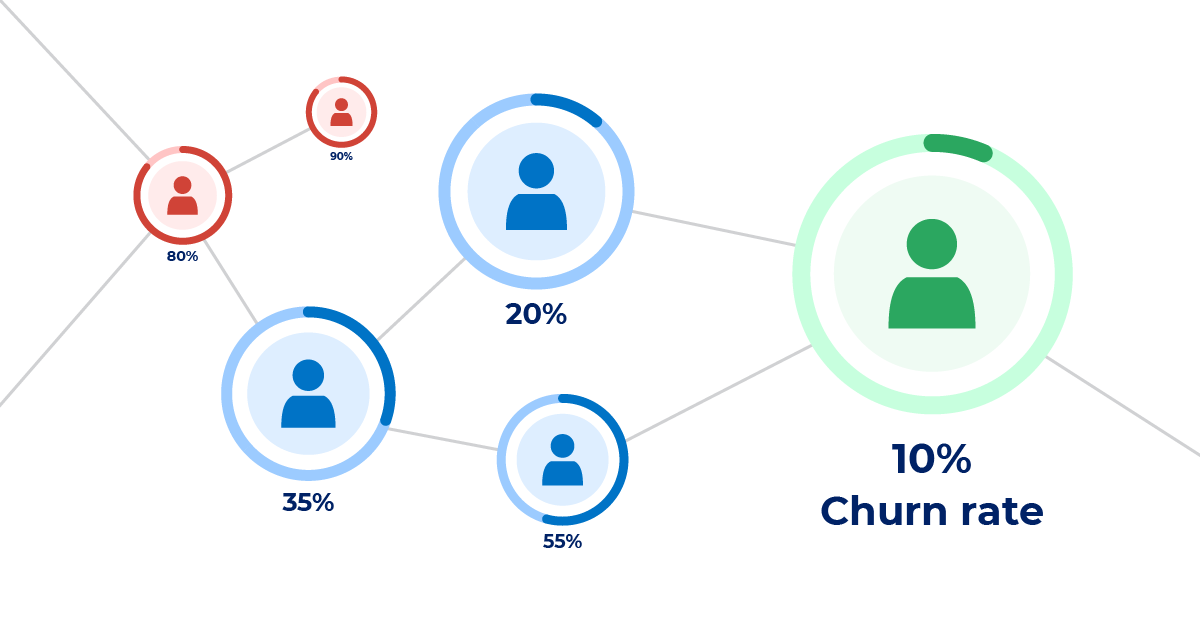
\includegraphics[width=\textwidth]{assets/first_page.png}
\end{figure}

\newpage

\tableofcontents

\newpage


\section{Motivation and Rationale}
It is obvious that the most important entity in a company or in a business is the customer. There are several aspects for managing a business, but nowadays, digital marketing is known as one of the best parts of a company.
They are focused on attracting customers to the product and services, but after this step we are dealing with another factor that is Churn Rate.
In fact there are several rival companies, and they are trying to offer better products or services in digital marketing and ads and that is why controlling the Churn Rate is really important.
It is possible that sometimes other factors have affected Churning users but in any situation If we are able to identify users that want to leave our services and predict it, we can break the churn by other techniques in digital marketing and remain users, so to speak we were able to break the churn. 
That is why this kind of research is really important for many companies.

\section{State of the Art}

\subsection{Predicting Customer Churn}
Churn prediction means detecting which customers are likely to leave a service or to cancel a subscription to a service. It is a critical prediction for many businesses because acquiring new clients often costs more than retaining existing ones. Once you can identify those customers that are at risk of canceling, you should know exactly what marketing action to take for each individual customer to maximize the chances that the customer will remain.\\
Different customers exhibit different behaviors and preferences, so they cancel their subscriptions for various reasons. It is critical, therefore, to proactively communicate with each of them in order to retain them in your customer list. You need to know which marketing action will be the most effective for each and every customer, and when it will be most effective.

\subsection{Why is it so important?}
Customer churn is a common problem across businesses in many sectors. If you want to grow as a company, you have to invest in acquiring new clients. Every time a client leaves, it represents a significant investment lost. Both time and effort need to be channeled into replacing them. Being able to predict when a client is likely to leave, and offer them incentives to stay, can offer huge savings to a business.\\
As a result, understanding what keeps customers engaged is extremely valuable knowledge, as it can help you to develop your retention strategies, and to roll out operational practices aimed at keeping customers from walking out the door.\\
Predicting churn is a fact of life for any subscription business, and even slight fluctuations in churn can have a significant impact on your bottom line. We need to know: “Is this customer going to leave us within X months?” Yes or No? It is a binary classification task.

\subsection{What are the main challenges?}
Churn prediction modelling techniques attempt to understand the precise customer behaviours and attributes that signal the risk and timing of customers leaving. It’s not a walk-in-the-park task so I mention just four points to consider.
\begin{itemize}
  \item[\textbf{1}] To succeed at retaining customers who are ready to abandon your business, Marketers and Customer Success experts must be able to predict in advance which customers are going to churn and set up a plan of marketing actions that will have the greatest retention impact on each customer. The key here is to be proactive and engage with these customers. While simple in theory, the realities involved with achieving this “proactive retention” goal are extremely challenging.
  \item[\textbf{2}] The accuracy of the technique is critical to the success of any proactive retention efforts. If the Marketer is unaware of a customer about to churn, no action will be taken to retain that customer.
  \item[\textbf{3}] Special retention-focused offers or incentives may be provided to happy, active customers, resulting in reduced revenues for no good reason.
  \item[\textbf{4}] Your churn prediction model should rely on (almost) real-time data to quantify the risk of churning, not on static data. Although you will be able to identify a certain percentage of at-risk customers with even static data, your predictions will be inaccurate. 
\end{itemize}
Bringing it all together, predicting customer churn is important. Effective action can be taken to retain the customer before it is too late. The ability to predict that a customer is at high risk of churning while there is still time to do something about it represents a huge additional potential revenue source for every online business.


\section{Objectives}
In short, we are trying to provide some model of Machine learning approaches to find a way to predict users that want to leave our service. It is clear that we are not able to have a certain answer about churn of a user because it depends on many factors, and we are just trying to find the most accurate approach to recognize users that want to leave service from a company. In detail, it can be said that if we are able to understand why a user leaves our service based on a series of parameters, then we can say that if a user in the future has parameters exactly with the profile of the user checked in the past, this user is probably Currently, they intend to leave the service.



\section{Methodology}
In this section, we will talk more about explaining technical issues and implementation details.

\subsection{Dataset}
One of the most famous and completed dataset that is available for public society is regarding Telco.
Telco is a company active in the field of telecommunications, and it is also an Internet Service provider.\\
They have published a dataset about 6 years ago, and it contains the rows (records) of 7043 users in 21 columns (features).The dataset is already available on the Kaggle, and it is accessible with this link:\\
\vspace{\baselineskip} \newline
https://www.kaggle.com/datasets/blastchar/telco-customer-churn/data
\vspace{\baselineskip} \newline
These years many people have worked on this dataset, and it can be helpful for us to avoid starting from scratch and have a better imagination to implement our approach by a logical and practical implementation.

\begin{table}[ht]
  \centering
  \small
  \begin{tabular}{|l|l|l|}
    \hline
    \textbf{Field} & \textbf{Values} & \textbf{Description} \\
    \hline
    customerID & String & Unique identifier \\
    gender & Male, Female & Gender \\
    SeniorCitizen & 1, 0 & Senior citizen status \\
    Partner & Yes, No & Has a partner \\
    Dependents & Yes, No & Has dependents \\
    Tenure & Numeric & Months with company \\
    PhoneService & Yes, No & Has phone service \\
    MultipleLines & Yes, No, No phone & Has multiple lines \\
    InternetService & DSL, Fiber optic, No & Internet service provider \\
    OnlineSecurity & Yes, No, No internet & Has online security \\
    OnlineBackup & Yes, No, No internet & Has online backup \\
    DeviceProtection & Yes, No, No internet & Has device protection \\
    TechSupport & Yes, No, No internet & Has tech support \\
    StreamingTV & Yes, No, No internet & Has streaming TV \\
    StreamingMovies & Yes, No, No internet & Has streaming movies \\
    Contract & Month-to-month, One year, Two year & Contract term \\
    PaperlessBilling & Yes, No & Paperless billing \\
    PaymentMethod & Electronic, Mailed, Bank transfer, Credit card & Payment method \\
    MonthlyCharges & Numeric & Monthly charges \\
    TotalCharges & Numeric & Total charges \\
    Churn & Yes, No & Churn status \\
    \hline
  \end{tabular}
  \caption{Description of Fields}
  \end{table}

\subsection{Methods and Algorithms}
In this project we have used 3 types of classification approaches in machine learning with 5 different implementations. Implementations in respectively are:
\begin{itemize}
  \item Preprocessing
  \item Split Data
  \item Principal Component Analysis (PCA)
  \item Bayes Decision Theory
  \item K-Nearest Neighbors 
  \item Support Vector Machine (SVM) with Linear, RBF and Sigmoid kernels
\end{itemize}
In the rest of this section we are going to disucss more about each methods and explain them.

\subsection{Preprocessing}
The main purpose of this step is just converting discrete values that are non-numerical to numbers and fulfill empty rows and clean data.

\subsection{Split Data}
It was predictable for us that we have to evaluate our results, and we have had just one dataset so we have tried to split data into two parts, 80 percent for train and 20 percent for test.

\subsection{Principal Component Analysis (PCA)}
As we have discussed in the 3.1 section there are 21 features in the dataset and in order to avoid dimensionality reduction and noise reduction, we applied PCA as a step of feature extraction.
There is an implementation in the Scikit-learn library, but we had to find the best number of components. For finding the number of components, we implemented some steps exactly like applying PCA on features. These steps are:
\begin{itemize}
  \item \textbf{Standardization:} Having smaller numbers and has a mean of 0 and a standard deviation of 1 for each feature.
  \item \textbf{Covariance Matrix Computation:} Calculate the covariance matrix to find relationships between variables.
  \item \textbf{Eigenvalue and Eigenvector Computation:} Find the covariance matrix's eigenvalues and eigenvectors.
  \item \textbf{Principal Components Selection:} Sort the eigenvalues in descending order, then select the top k eigenvalues.
  \item \textbf{Data Transformation:} Translates the initial data onto the newly specified feature space that the major components have defined.
\end{itemize}
Finally, we have chosen 3 of the biggest eigenvalues with respectively numbers 1, 1 and 0.99, and we set the number of components equal to 3.

\subsection{Bayes Decision Theory}
For applying Naive Bayes on our data, we have chosen Gaussian Naive Bayes. Gaussian Naive Bayes is a variant of the Naive Bayes algorithm, but it works on values that follow a Gaussian (normal) distribution. As we have seen in the PCA step, we have normalized our data so we can apply Gaussian Naive Bayes.
Finally, for finding probabilistic data we have applied Naive Bayes on our train data.

\subsection{K-Nearest Neighbors}
For implementation of K-Nearest Neighbors we were dealing with the k number. In many cases we can ask for a K number from a domain expert but despite many searches there was no reasonable K number so we have decided to find the best K as train and evaluation for each K in a loop. Also we have tried to store standard deviation for each k.\\
Finally, we have found the best accuracy is with 0.7799858055358411 with k= 6.

\subsection{Support Vector Machine (SVM)}
In order to implement SVM, we have used Scikit like previous steps. We have tried SVM by 3 kernels that are Linear, Sigmoid and RBF. All 3 chapters are implemented totally the same but for RBF we have had a problem about zero division, and we had to balance the class-weight in parameters.



\section{Experiments \& Results}
For producing results and having comparisons between the different approaches and algorithms, we have tried to make some evaluation for each approach. As we have mentioned in section 3.4 we have split our data for train and test and dimensions of them are respectively 80 percent and 20 percent.\\
Furthermore, we have checked accuracy score and calculated Precision, Recall and F1 scores for remain and churn users separately. In continuation, we are going to compare the results of each approach.

\subsection{Confsion Matrix}
In a 2 by 2 confusion matrix of our problem there are 4 sections or 4 factors.
\begin{itemize}
  \item \textbf{True Positive:} This index shows the number of users who wanted to leave, and we predicted that they would leave.
  \item \textbf{True Negative:} This index represents the number of users who wanted to leave, and we predicted they would not.
  \item \textbf{False Positive:} This index shows the number of users who did not want to leave, and we predicted that they would.
  \item \textbf{False Negative:} This index shows the number of users who did not want to go, and we predicted that they would not go.
\end{itemize}

\begin{table}[ht]
  \centering
\begin{tabular}{|l|l|l|}
  \hline
  & \text{Predicted Positive} & \text{Predicted Negative} \\
  \hline
  \text{Actual Positive} & TP & FN \\
  \hline
  \text{Actual Negative} & FP & TN \\
  \hline
\end{tabular}
\end{table}

\newpage
As conseences we are going to calculate our scores with this formulas:\\
\vspace{\baselineskip}

Accuracy:
\[
\text{Accuracy} = \frac{TP + TN}{TP + FP + FN + TN}
\]

Precision:
\[
\text{Precision} = \frac{TP}{TP + FP}
\]

Recall:
\[
\text{Recall} = \frac{TP}{TP + FN}
\]

F1 Score:
\[
\text{F1 Score} = 2 \times \frac{\text{Precision} \times \text{Recall}}{\text{Precision} + \text{Recall}}
\]

\vspace{\baselineskip}

\subsubsection{Bayes decision theory Matrix}
\begin{table}[ht]
  \large
  \centering
\begin{tabular}{|l|l|}
  \hline
  191 & 193\\
  \hline
  169 & 866\\
  \hline
\end{tabular}
\end{table}
\begin{itemize}
  \item \textbf{Classifier accuracy:} 75.02\%
  \item \textbf{Precision for remain:} 83\%
  \item \textbf{Precision for chrun:} 53\%
  \item \textbf{Recall for remain:} 84\%
  \item \textbf{Recall for churn:} 51\%
  \item \textbf{F1 for remain:} 83\%
  \item \textbf{F1 for churn:} 52\%
\end{itemize}

\newpage

\subsubsection{K-Nearest Neighbors Matrix}
\begin{table}[ht]
  \large
  \centering
\begin{tabular}{|l|l|}
  \hline
  141 & 233\\
  \hline
  77 & 958\\
  \hline
\end{tabular}
\end{table}
\begin{itemize}
  \item \textbf{Classifier accuracy:} 78\%
  \item \textbf{Precision for remain:} 80\%
  \item \textbf{Precision for chrun:} 65\%
  \item \textbf{Recall for remain:} 93\%
  \item \textbf{Recall for churn:} 38\%
  \item \textbf{F1 for remain:} 86\%
  \item \textbf{F1 for churn:} 48\%
\end{itemize}

\vspace{\baselineskip}

\subsubsection{SVM with Linear kernel Matrix}
\begin{table}[ht]
  \large
  \centering
\begin{tabular}{|l|l|}
  \hline
  157 & 217\\
  \hline
  108 & 927\\
  \hline
\end{tabular}
\end{table}
\begin{itemize}
  \item \textbf{Classifier accuracy:} 76\%
  \item \textbf{Precision for remain:} 81\%
  \item \textbf{Precision for chrun:} 59\%
  \item \textbf{Recall for remain:} 90\%
  \item \textbf{Recall for churn:} 42\%
  \item \textbf{F1 for remain:} 85\%
  \item \textbf{F1 for churn:} 49\%
\end{itemize}

\newpage

\subsubsection{SVM with RBF kernel Matrix}
\begin{table}[ht]
  \large
  \centering
\begin{tabular}{|l|l|}
  \hline
  239 & 135\\
  \hline
  296 & 739\\
  \hline
\end{tabular}
\end{table}
\begin{itemize}
  \item \textbf{Classifier accuracy:} 69.41\%
  \item \textbf{Precision for remain:} 85\%
  \item \textbf{Precision for chrun:} 45\%
  \item \textbf{Recall for remain:} 71\%
  \item \textbf{Recall for churn:} 64\%
  \item \textbf{F1 for remain:} 77\%
  \item \textbf{F1 for churn:} 53\%
\end{itemize}

\vspace{\baselineskip}

\subsubsection{SVM with Sigmoid kernel Matrix}
\begin{table}[ht]
  \large
  \centering
\begin{tabular}{|l|l|}
  \hline
  150 & 224\\
  \hline
  227 & 808\\
  \hline
\end{tabular}
\end{table}
\begin{itemize}
  \item \textbf{Classifier accuracy:} 67.99\%
  \item \textbf{Precision for remain:} 78\%
  \item \textbf{Precision for chrun:} 40\%
  \item \textbf{Recall for remain:} 78\%
  \item \textbf{Recall for churn:} 40\%
  \item \textbf{F1 for remain:} 78\%
  \item \textbf{F1 for churn:} 40\%
\end{itemize}

\newpage



\section{Conclusions}
This is obvious that the highest accuracy is related to KNN method, but we know the most important factor for these kinds of project is detecting users who want to leave the service, and we should recognize them, these kinds of users are showing by True Positive (TP) so with another glance we can find an approach to calculate and find the best method. We can calculate average of churn evaluations and find the best, so the best approach in descending order are:
\begin{itemize}
  \item \textbf{SVM (RBF):} 54\%
  \item \textbf{Bayes:} 52\%
  \item \textbf{KNN:} 50.33\%
  \item \textbf{SVM (Linear):} 50\%
  \item \textbf{SVM (Sigmoid):} 40\%
\end{itemize}
So we can say SVM with RBF kernel has the most correctness prediction about the churn users despite all the results being so closed, but SVM with Sigmoid kernel has the worst result with a significant gap in comparison with others.\\
And another important factor is preference, as we have seen all the methods have had really good preformance on our dataset except SVM with Linear kernel that takes some minutes for training the model.

\newpage
\section{Bibliography or References}
\vspace{\baselineskip}
\textbf{The most important references that we have used to implement approaches:}
\vspace{\baselineskip}
\newline
www.scikit\-learn.org\\
www.kaggle.com/datasets/blastchar/telco-customer-churn/data\\
www.medium.com/@bhattbhavesh91/the-mystery-of-n-components-in-pca-a0431ee995be
\vspace{2cm}
\newline
\textbf{Tools that are used for writing this report:}
\vspace{\baselineskip}
\newline
www.latex-project.org \\
www.docs.google.com\\
www.languagetool.org




\end{document}